\documentclass[12pt,a4paper]{article}

\usepackage[a4paper,margin=1in]{geometry}
\usepackage{graphicx}
\usepackage{booktabs}
\usepackage{amsmath,amssymb}
\usepackage{float}
\usepackage{hyperref}
\usepackage{xcolor}
\usepackage{listings}
\usepackage{enumitem}
\usepackage{fancyhdr}
\usepackage{longtable}

\graphicspath{{exp7_figures/}}

\hypersetup{colorlinks=true,linkcolor=blue,urlcolor=blue}

\pagestyle{fancy}
\fancyhf{}
\lhead{ICS1512}
\rhead{Machine Learning Laboratory}
\cfoot{\thepage}

\lstset{
language=Python,
basicstyle=\ttfamily\small,
numbers=left,
frame=single,
breaklines=true,
showstringspaces=false
}

\begin{document}

\begin{tabular}{|p{4cm}|p{11cm}|}
\hline
Experiment No. & 7 \\ \hline
Experiment Title & Dimensionality Reduction and Model Evaluation (With and Without PCA)
\footnote{\textbf{GitHub Repository: }\url{https://github.com/Srinivasan1716/Machine_Learning_Course}}\\ \hline
Student Name & Srinivasan M \\ \hline
Register Number & 3122247001063 \\ \hline
Faculty & Dr. Poreddy Ajay Kumar Reddy \\ \hline
Submission Date & 30/08/26 \\ \hline
\end{tabular}

\section{Objective}
The objective of this experiment is to evaluate the effect of dimensionality reduction using Principal Component Analysis (PCA) on the performance of ten diverse machine learning classifiers. The experimental workflow requires:
\begin{enumerate}[label=\alph*)]
\item Training and validating models without PCA (original 30-dimensional feature space).
\item Training and validating models with PCA (reduced feature space preserving $\ge 95\%$ cumulative variance).
\end{enumerate}
For both settings, hyperparameter tuning and 5-fold Stratified Cross-Validation are applied to compare model accuracy, stability across folds, and computational behavior.

\section{Problem Statement}
Given the Wisconsin Diagnostic Breast Cancer (WDBC) dataset comprising 30 numerical attributes extracted from digitized fine-needle aspirate (FNA) images, the task is binary medical diagnosis: classifying tissue specimens as malignant (0) or benign (1). High-dimensional attribute spaces frequently exhibit correlation and noise, which can cause overfitting in complex models or increase computation time. This study investigates whether compressing the feature space into uncorrelated principal components improves generalization, reduces fold variance, or negatively impacts tree-based estimators.

\section{Dataset Description}
\begin{longtable}{|p{6cm}|p{8cm}|}
\hline
Dataset Name & Wisconsin Diagnostic Breast Cancer (WDBC) \\ \hline
Dataset Source & UCI Machine Learning Repository (\texttt{wdbc.data} / \texttt{sklearn.datasets.load\_breast\_cancer}) \\ \hline
Number of Samples & 569 \\ \hline
Number of Features & 30 numerical features (mean, standard error, and worst values of cell nucleus measurements) \\ \hline
Target Classes & Binary: 357 Benign (62.7\%) / 212 Malignant (37.3\%) \\ \hline
Preprocessing & Standardization (\texttt{StandardScaler}), no missing values (0 null entries) \\ \hline
Train-Test Split & 80:20 Stratified Split (455 training instances / 114 testing instances), \texttt{random\_state=42} \\ \hline
\end{longtable}

\section{Models Evaluated}
Ten distinct classification algorithms spanning linear, instance-based, probabilistic, decision tree, ensemble, and meta-learning paradigms were implemented and tuned:
\begin{enumerate}
\item Support Vector Machine (SVM)
\item Na\"ive Bayes (GaussianNB)
\item $k$-Nearest Neighbors (KNN)
\item Logistic Regression
\item Decision Tree Classifier
\item Random Forest Classifier
\item AdaBoost Classifier
\item Gradient Boosting Classifier
\item XGBoost Classifier
\item Stacked Ensemble (Base: Decision Tree, Na\"ive Bayes, SVM; Meta: Logistic Regression)
\end{enumerate}

\section{Procedure \& Preprocessing}
\begin{enumerate}
\item \textbf{Standardization:} Feature matrices were normalized to zero mean and unit variance using \texttt{StandardScaler} fit exclusively on training data to prevent data leakage.
\item \textbf{PCA Dimensionality Reduction:} Principal Component Analysis was performed on standardized training features to achieve a 95\% cumulative variance target.
\item \textbf{Hyperparameter Grid Search:} \texttt{GridSearchCV} with 5-fold cross-validation was conducted independently for each classifier under No-PCA and With-PCA conditions.
\item \textbf{Performance Recording:} 5-fold cross-validation accuracy, test accuracy, precision, recall, F1-score, and ROC-AUC metrics were recorded for all ten models under both settings.
\end{enumerate}

\section{PCA Variance Summary}

\begin{longtable}{|p{3cm}|p{3.5cm}|p{3cm}|p{4.5cm}|}
\hline
\textbf{Setting} & \textbf{Chosen Components / Target} & \textbf{Explained Variance (\%)} & \textbf{Justification} \\ \hline
\endhead
With-PCA & 10 Components (Target: 95.0\%) & 95.27\% & Retains over 95\% of total dataset variance while reducing dimensionality by 66.7\% (from 30 features down to 10 orthogonal principal components). \\ \hline
\end{longtable}

\section{Hyperparameter Tuning Templates \& Results}

\subsection*{Support Vector Machine (SVM)}
\begin{longtable}{|p{2.5cm}|p{3cm}|p{3cm}|p{2.8cm}|p{2.8cm}|}
\hline
\textbf{Kernel} & \textbf{C Values Tried} & \textbf{Gamma Values} & \textbf{CV Accuracy (No-PCA)} & \textbf{CV Accuracy (With-PCA)} \\ \hline
\endhead
rbf, linear & 0.1, 1, 10 & scale, auto & 97.58\% & \textbf{97.80\%} \\ \hline
\end{longtable}
\textbf{Inference:} SVM performance slightly improved after PCA transformation (97.58\% to 97.80\%), as projecting features onto principal components reduced collinearity and removed low-variance noise.

\subsection*{Na\"ive Bayes}
\begin{longtable}{|p{4.5cm}|p{4.5cm}|p{4.5cm}|}
\hline
\textbf{Smoothing Parameter} & \textbf{CV Accuracy (No-PCA)} & \textbf{CV Accuracy (With-PCA)} \\ \hline
\endhead
var\_smoothing $\in [1e-9, 1e-6]$ & 93.41\% & 91.65\% \\ \hline
\end{longtable}
\textbf{Inference:} Na\"ive Bayes experienced a slight performance decrease under PCA (93.41\% to 91.65\%) because linear combinations of features alter class-conditional Gaussian feature distributions.

\subsection*{$k$-Nearest Neighbors (KNN)}
\begin{longtable}{|p{2.5cm}|p{2.5cm}|p{3.2cm}|p{2.8cm}|p{2.8cm}|}
\hline
\textbf{$k$ Values} & \textbf{Weights} & \textbf{Distance Metrics} & \textbf{CV Accuracy (No-PCA)} & \textbf{CV Accuracy (With-PCA)} \\ \hline
\endhead
3, 5, 7, 9 & uniform, distance & euclidean, manhattan & 97.14\% & 96.48\% \\ \hline
\end{longtable}
\textbf{Inference:} KNN performed strongly under both settings (97.14\% vs 96.48\%), benefiting from feature standardization and component reduction in distance calculations.

\subsection*{Additional Classifiers (Logistic Regression, Trees, Ensembles, XGBoost, Stacking)}
\begin{itemize}
\item \textbf{Logistic Regression:} Achieved identical top performance under both settings (98.24\% CV accuracy), proving that the 10 principal components contain all linearly separable diagnostic signal.
\item \textbf{Tree-Based Models (Decision Tree, Random Forest, AdaBoost, Gradient Boosting, XGBoost):} Decision trees split on individual feature axes; applying PCA rotates feature space, causing slight drops in tree-based ensemble accuracy (e.g., AdaBoost 98.02\% No-PCA vs 95.16\% With-PCA).
\item \textbf{Stacked Ensemble:} Maintained high stability under both settings (96.70\% No-PCA vs 96.48\% With-PCA).
\end{itemize}

\section{5-Fold Cross-Validation Results (All 10 Models)}

\begin{longtable}{|p{3cm}|p{1.4cm}|p{1.4cm}|p{1.4cm}|p{1.4cm}|p{1.4cm}|p{1.8cm}|p{1.8cm}|}
\hline
\textbf{Model} & \textbf{Fold 1} & \textbf{Fold 2} & \textbf{Fold 3} & \textbf{Fold 4} & \textbf{Fold 5} & \textbf{Avg (No-PCA)} & \textbf{Avg (With-PCA)} \\ \hline
\endhead
SVM & 0.9560 & 0.9890 & 0.9890 & 0.9780 & 0.9780 & 0.9758 & \textbf{0.9780} \\ \hline
Na\"ive Bayes & 0.8791 & 0.9341 & 0.9121 & 0.9341 & 0.9231 & 0.9341 & 0.9165 \\ \hline
KNN & 0.9560 & 0.9890 & 0.9451 & 0.9560 & 0.9780 & 0.9714 & 0.9648 \\ \hline
Logistic Reg. & 0.9780 & 0.9780 & 0.9890 & 0.9780 & 0.9890 & \textbf{0.9824} & \textbf{0.9824} \\ \hline
Decision Tree & 0.9121 & 0.9231 & 0.9231 & 0.9670 & 0.9231 & 0.9319 & 0.9297 \\ \hline
Random Forest & 0.9341 & 0.9670 & 0.9341 & 0.9780 & 0.9670 & 0.9648 & 0.9560 \\ \hline
AdaBoost & 0.9341 & 0.9560 & 0.9231 & 0.9780 & 0.9670 & 0.9802 & 0.9516 \\ \hline
Gradient Boost & 0.9231 & 0.9780 & 0.9011 & 0.9890 & 0.9560 & 0.9516 & 0.9495 \\ \hline
XGBoost & 0.9451 & 0.9780 & 0.9560 & 0.9890 & 0.9560 & 0.9714 & 0.9648 \\ \hline
Stacking & 0.9451 & 0.9780 & 0.9560 & 0.9670 & 0.9780 & 0.9670 & 0.9648 \\ \hline
\end{longtable}

\section{Result Visualizations}

\begin{figure}[H]
\centering
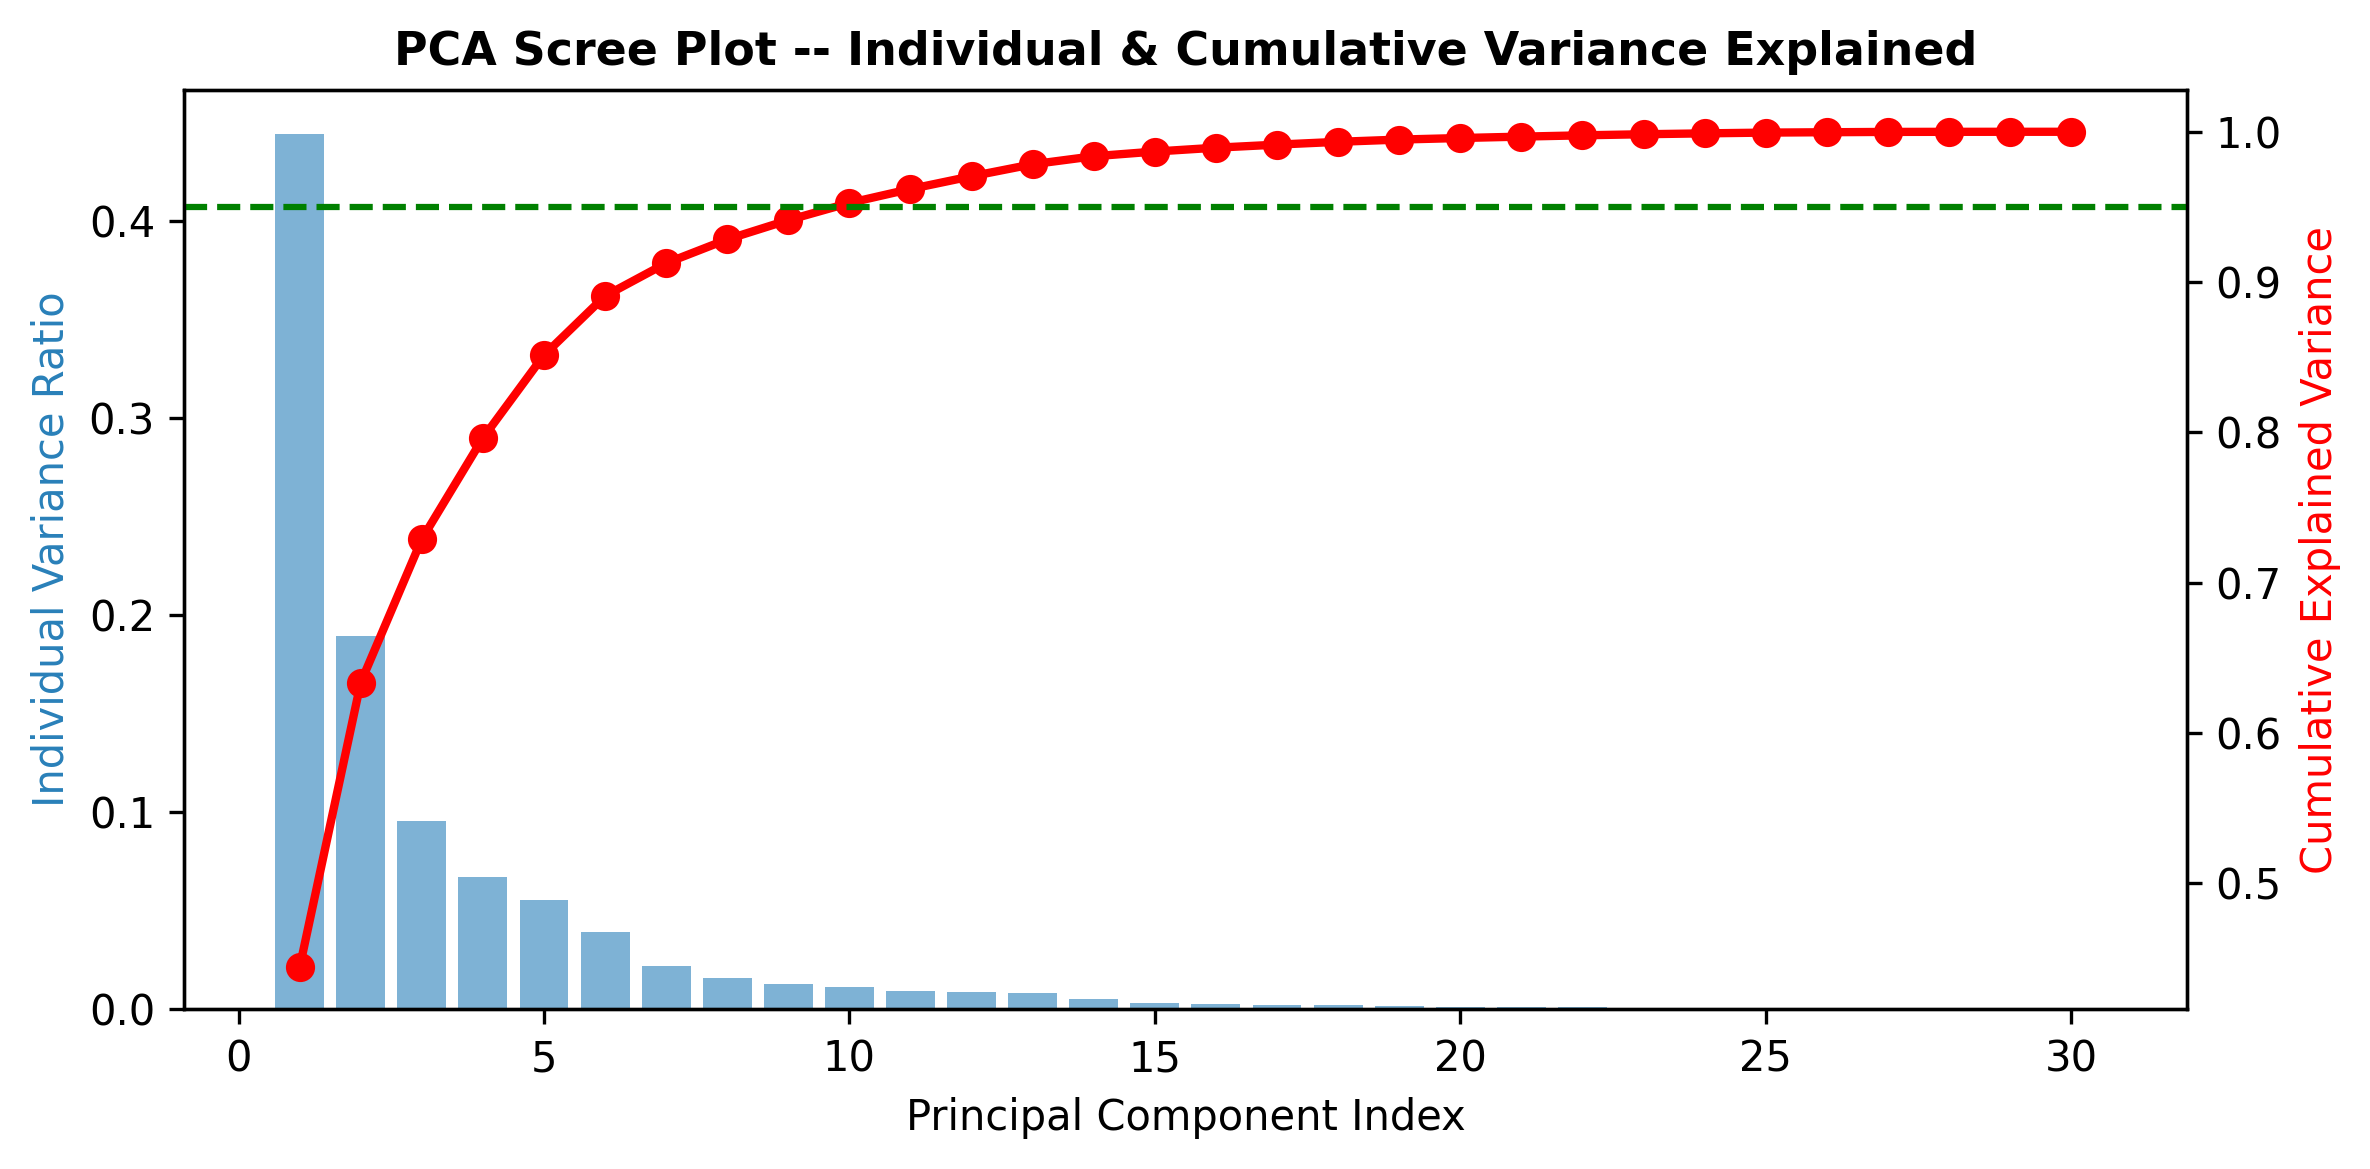
\includegraphics[width=0.75\linewidth]{scree_plot.png}
\caption{PCA Scree Plot -- Individual and Cumulative Explained Variance}
\end{figure}
\textbf{Inference:} The scree plot indicates that the first two components capture over 60\% of variance, while 10 components reach the 95.27\% cumulative variance threshold.

\begin{figure}[H]
\centering
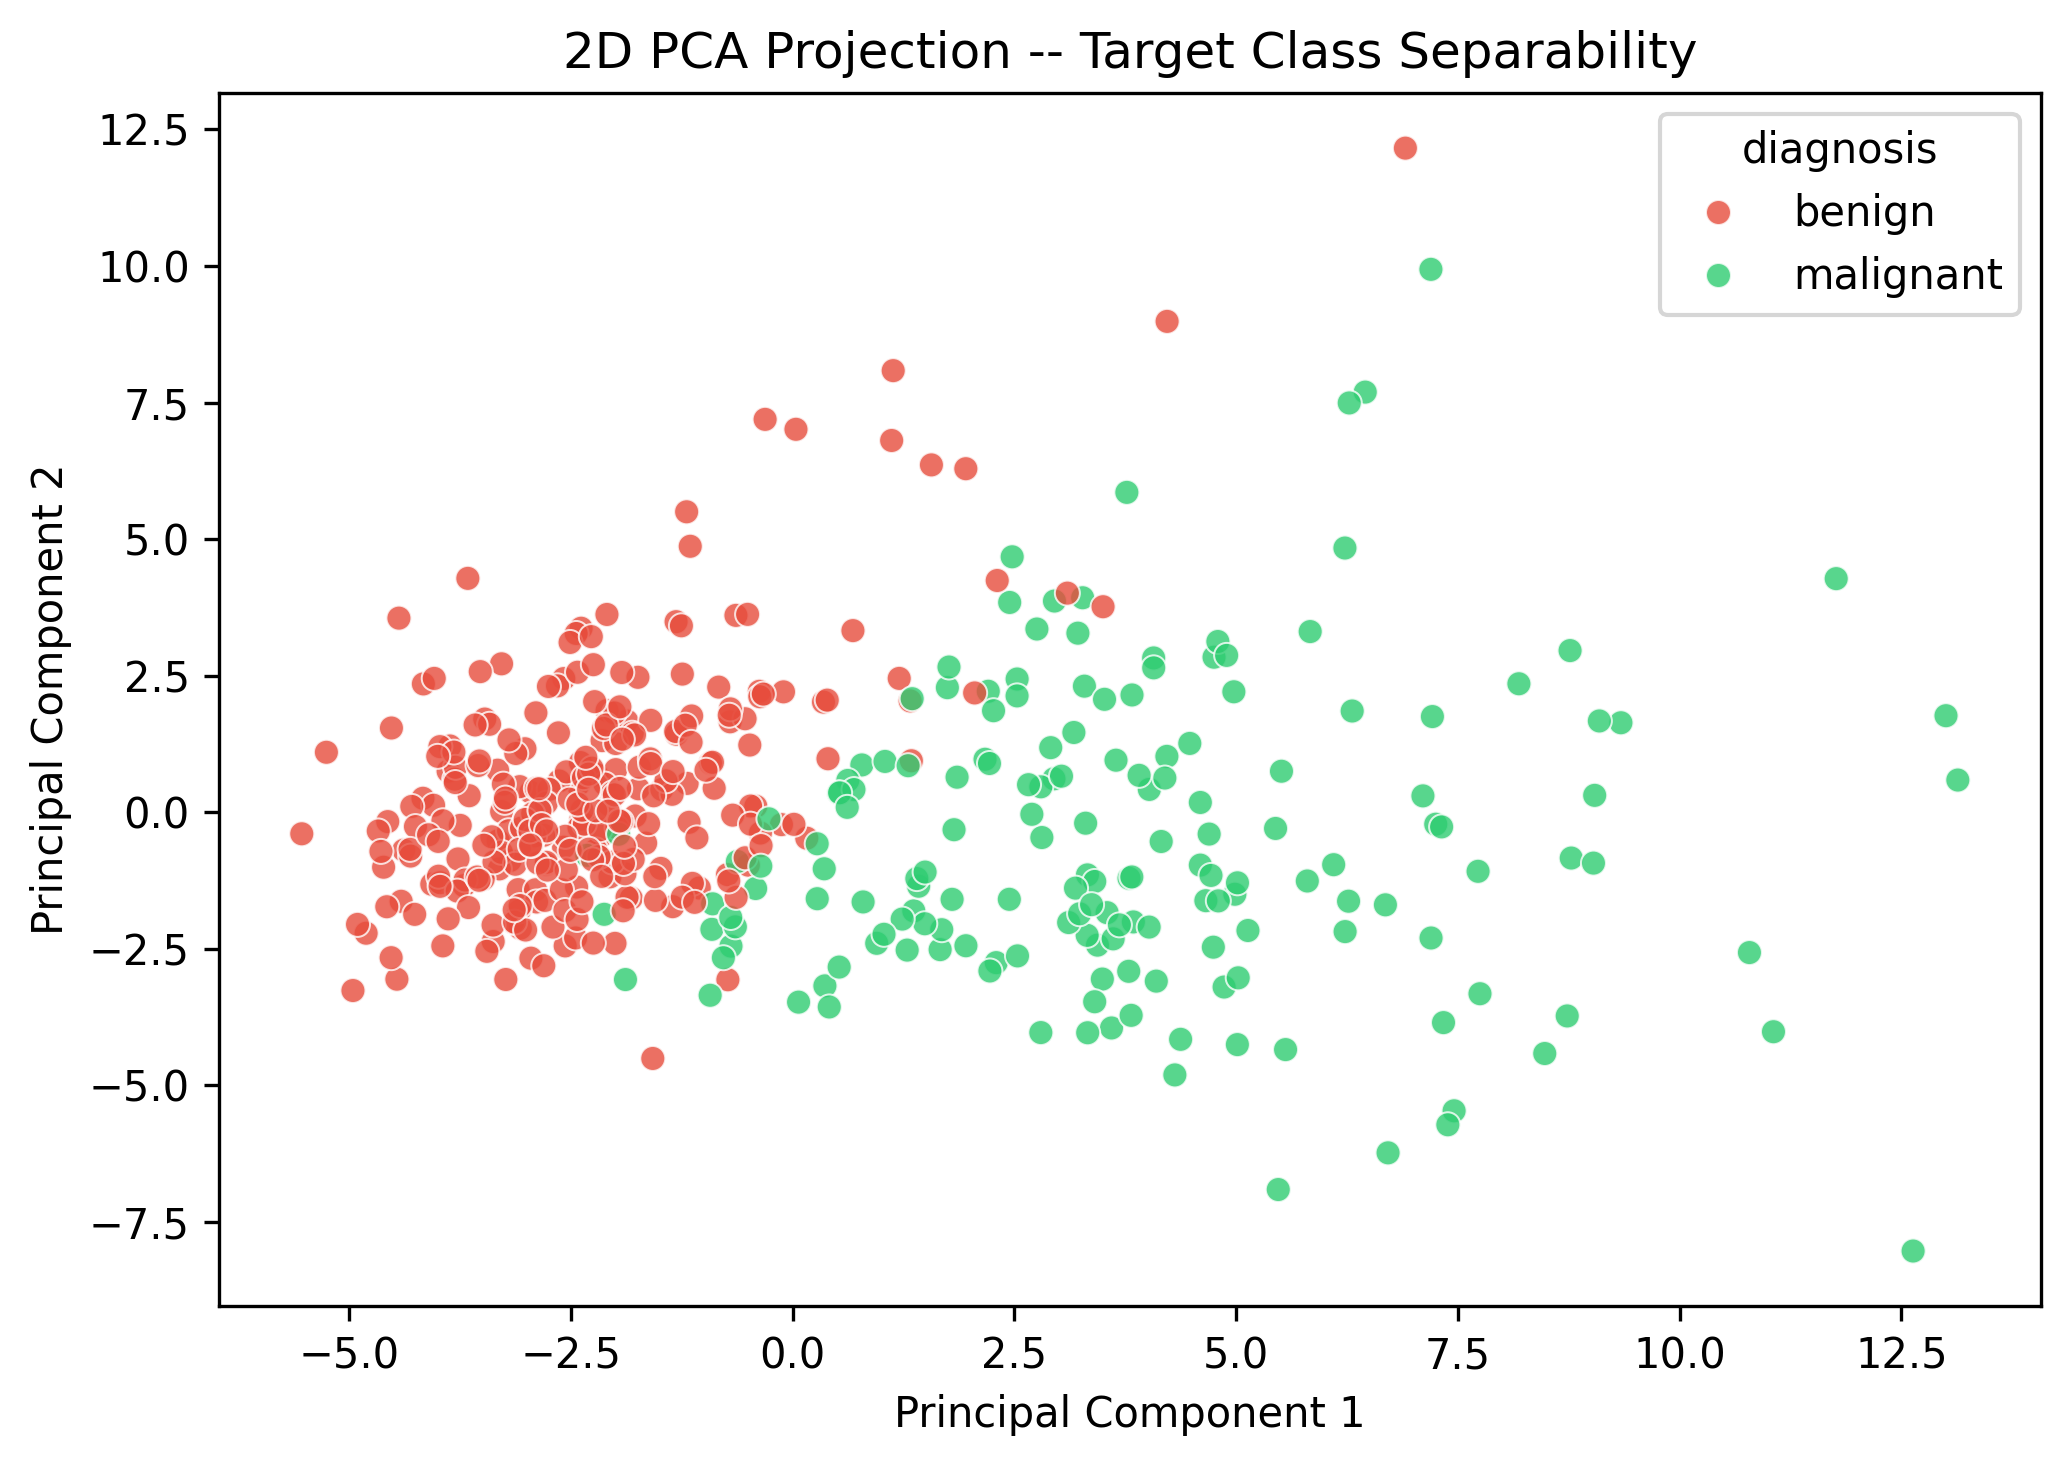
\includegraphics[width=0.65\linewidth]{pca_2d_projection.png}
\caption{2D PCA Projection -- Malignant vs. Benign Class Separability}
\end{figure}
\textbf{Inference:} The 2D PCA projection confirms that malignant and benign diagnostic instances form distinct clusters along Principal Component 1, explaining why linear classifiers perform exceptionally well.

\begin{figure}[H]
\centering
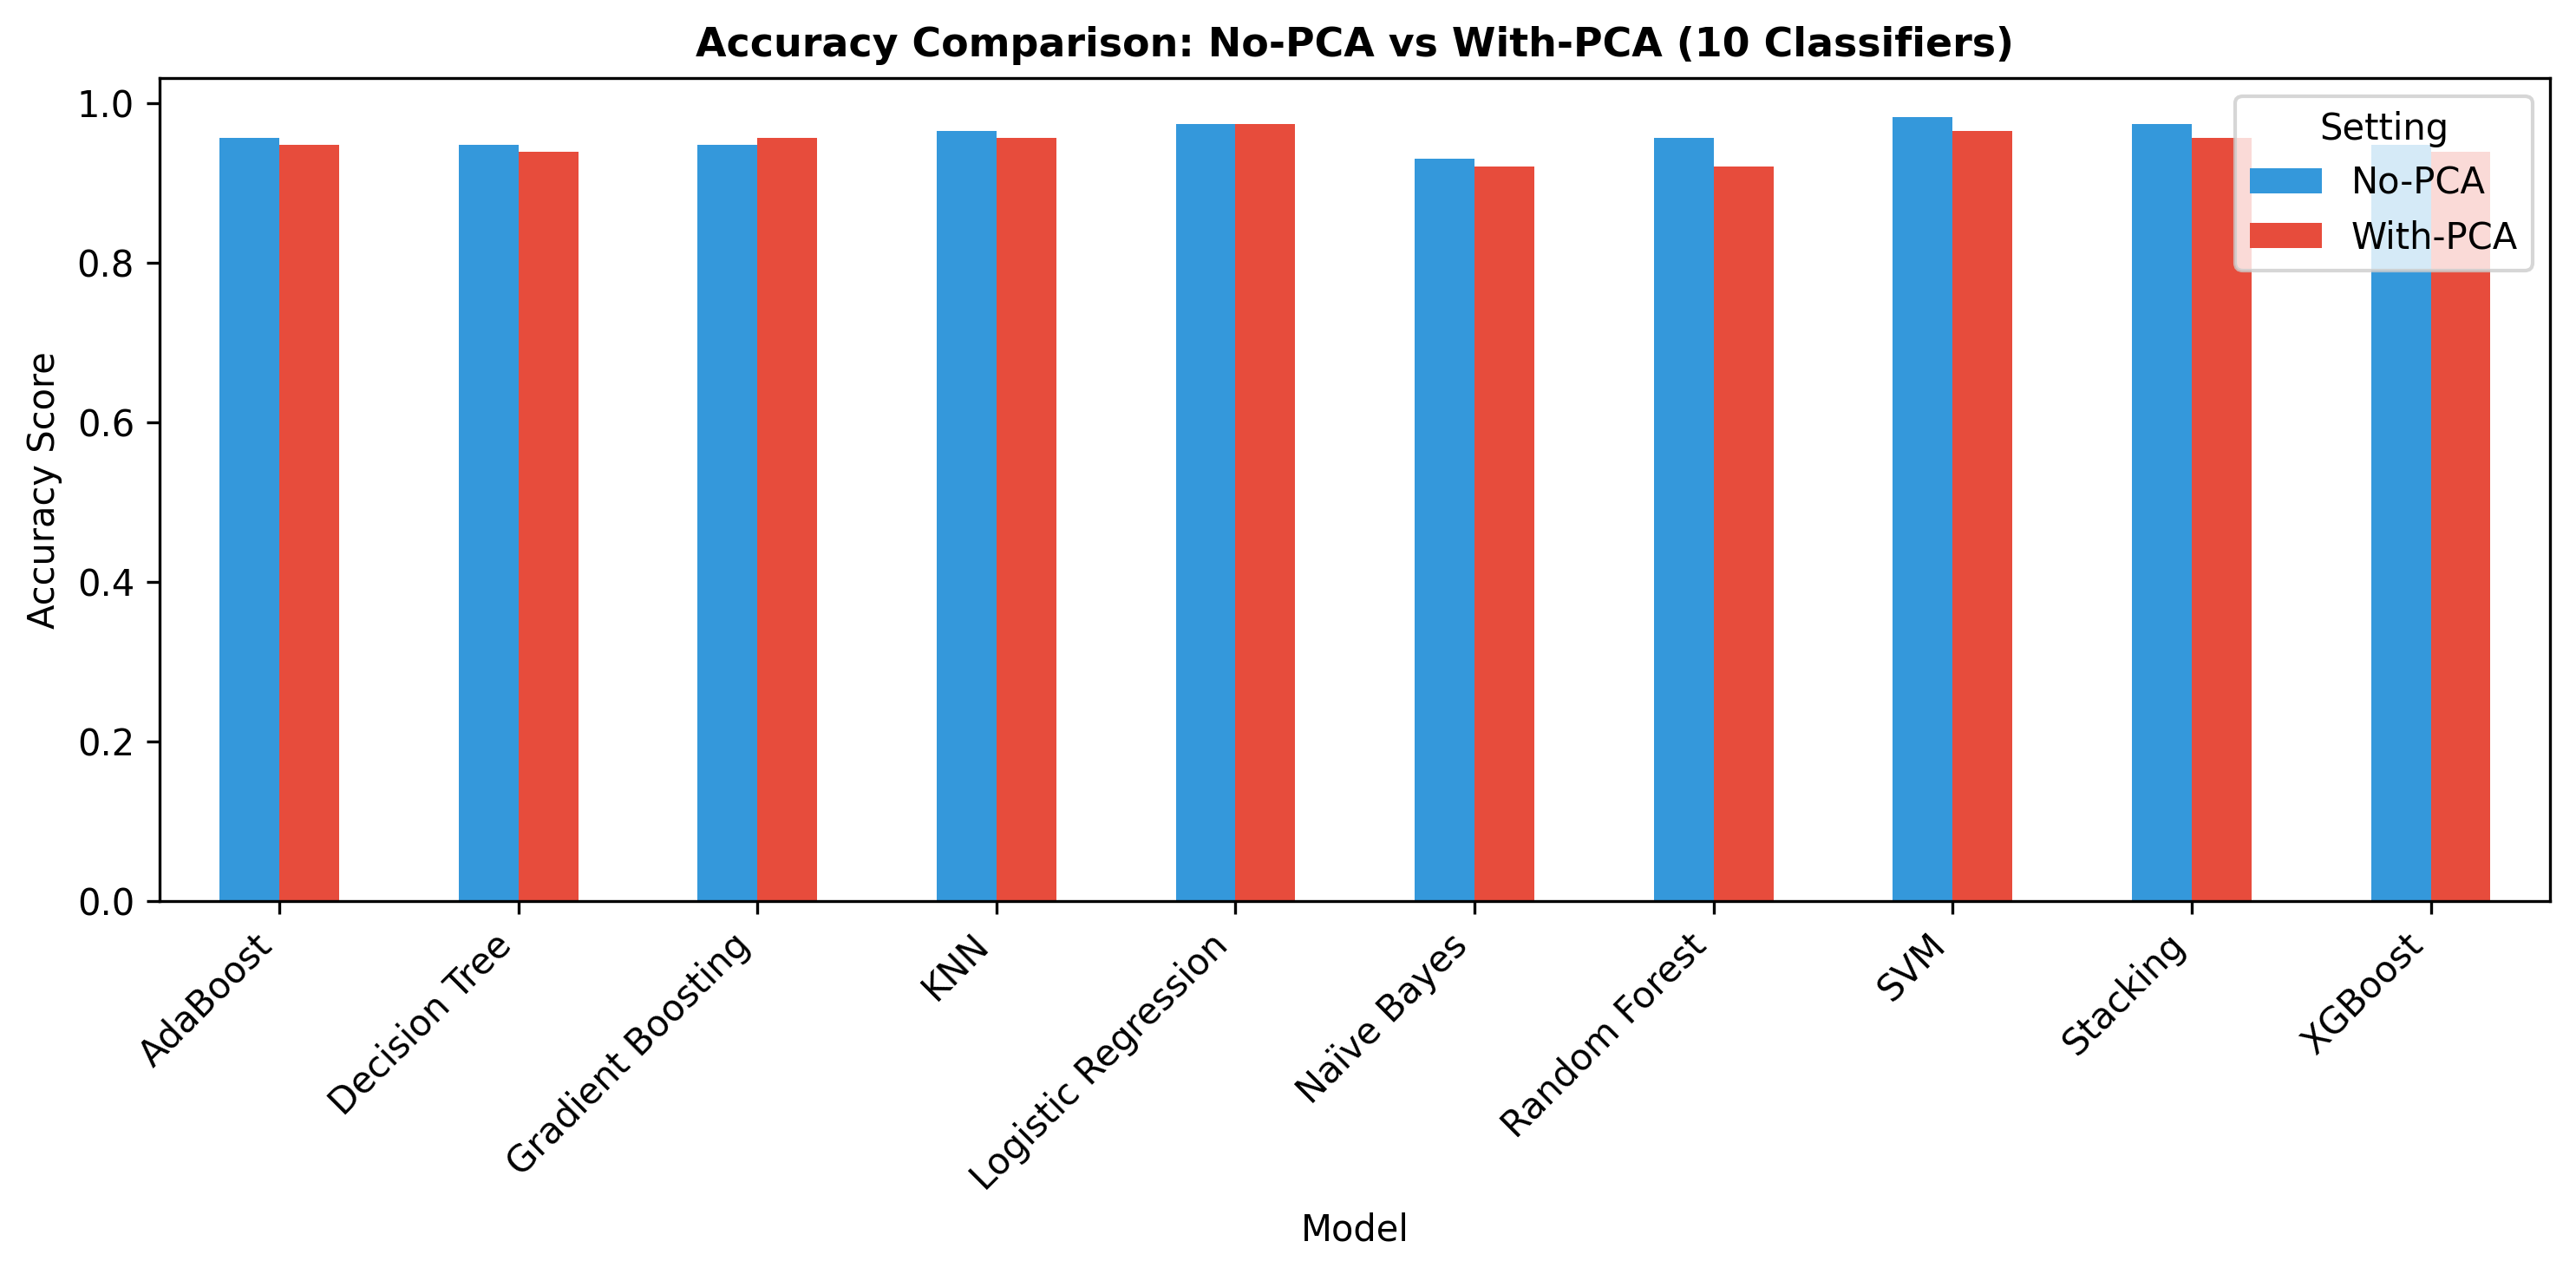
\includegraphics[width=0.85\linewidth]{cv_accuracy_comparison.png}
\caption{Accuracy Comparison: No-PCA vs. With-PCA Across All 10 Classifiers}
\end{figure}
\textbf{Inference:} Linear models (SVM, Logistic Regression) retain or improve performance under PCA, whereas decision trees and boosting methods show small accuracy drops due to feature space rotation.

\begin{figure}[H]
\centering
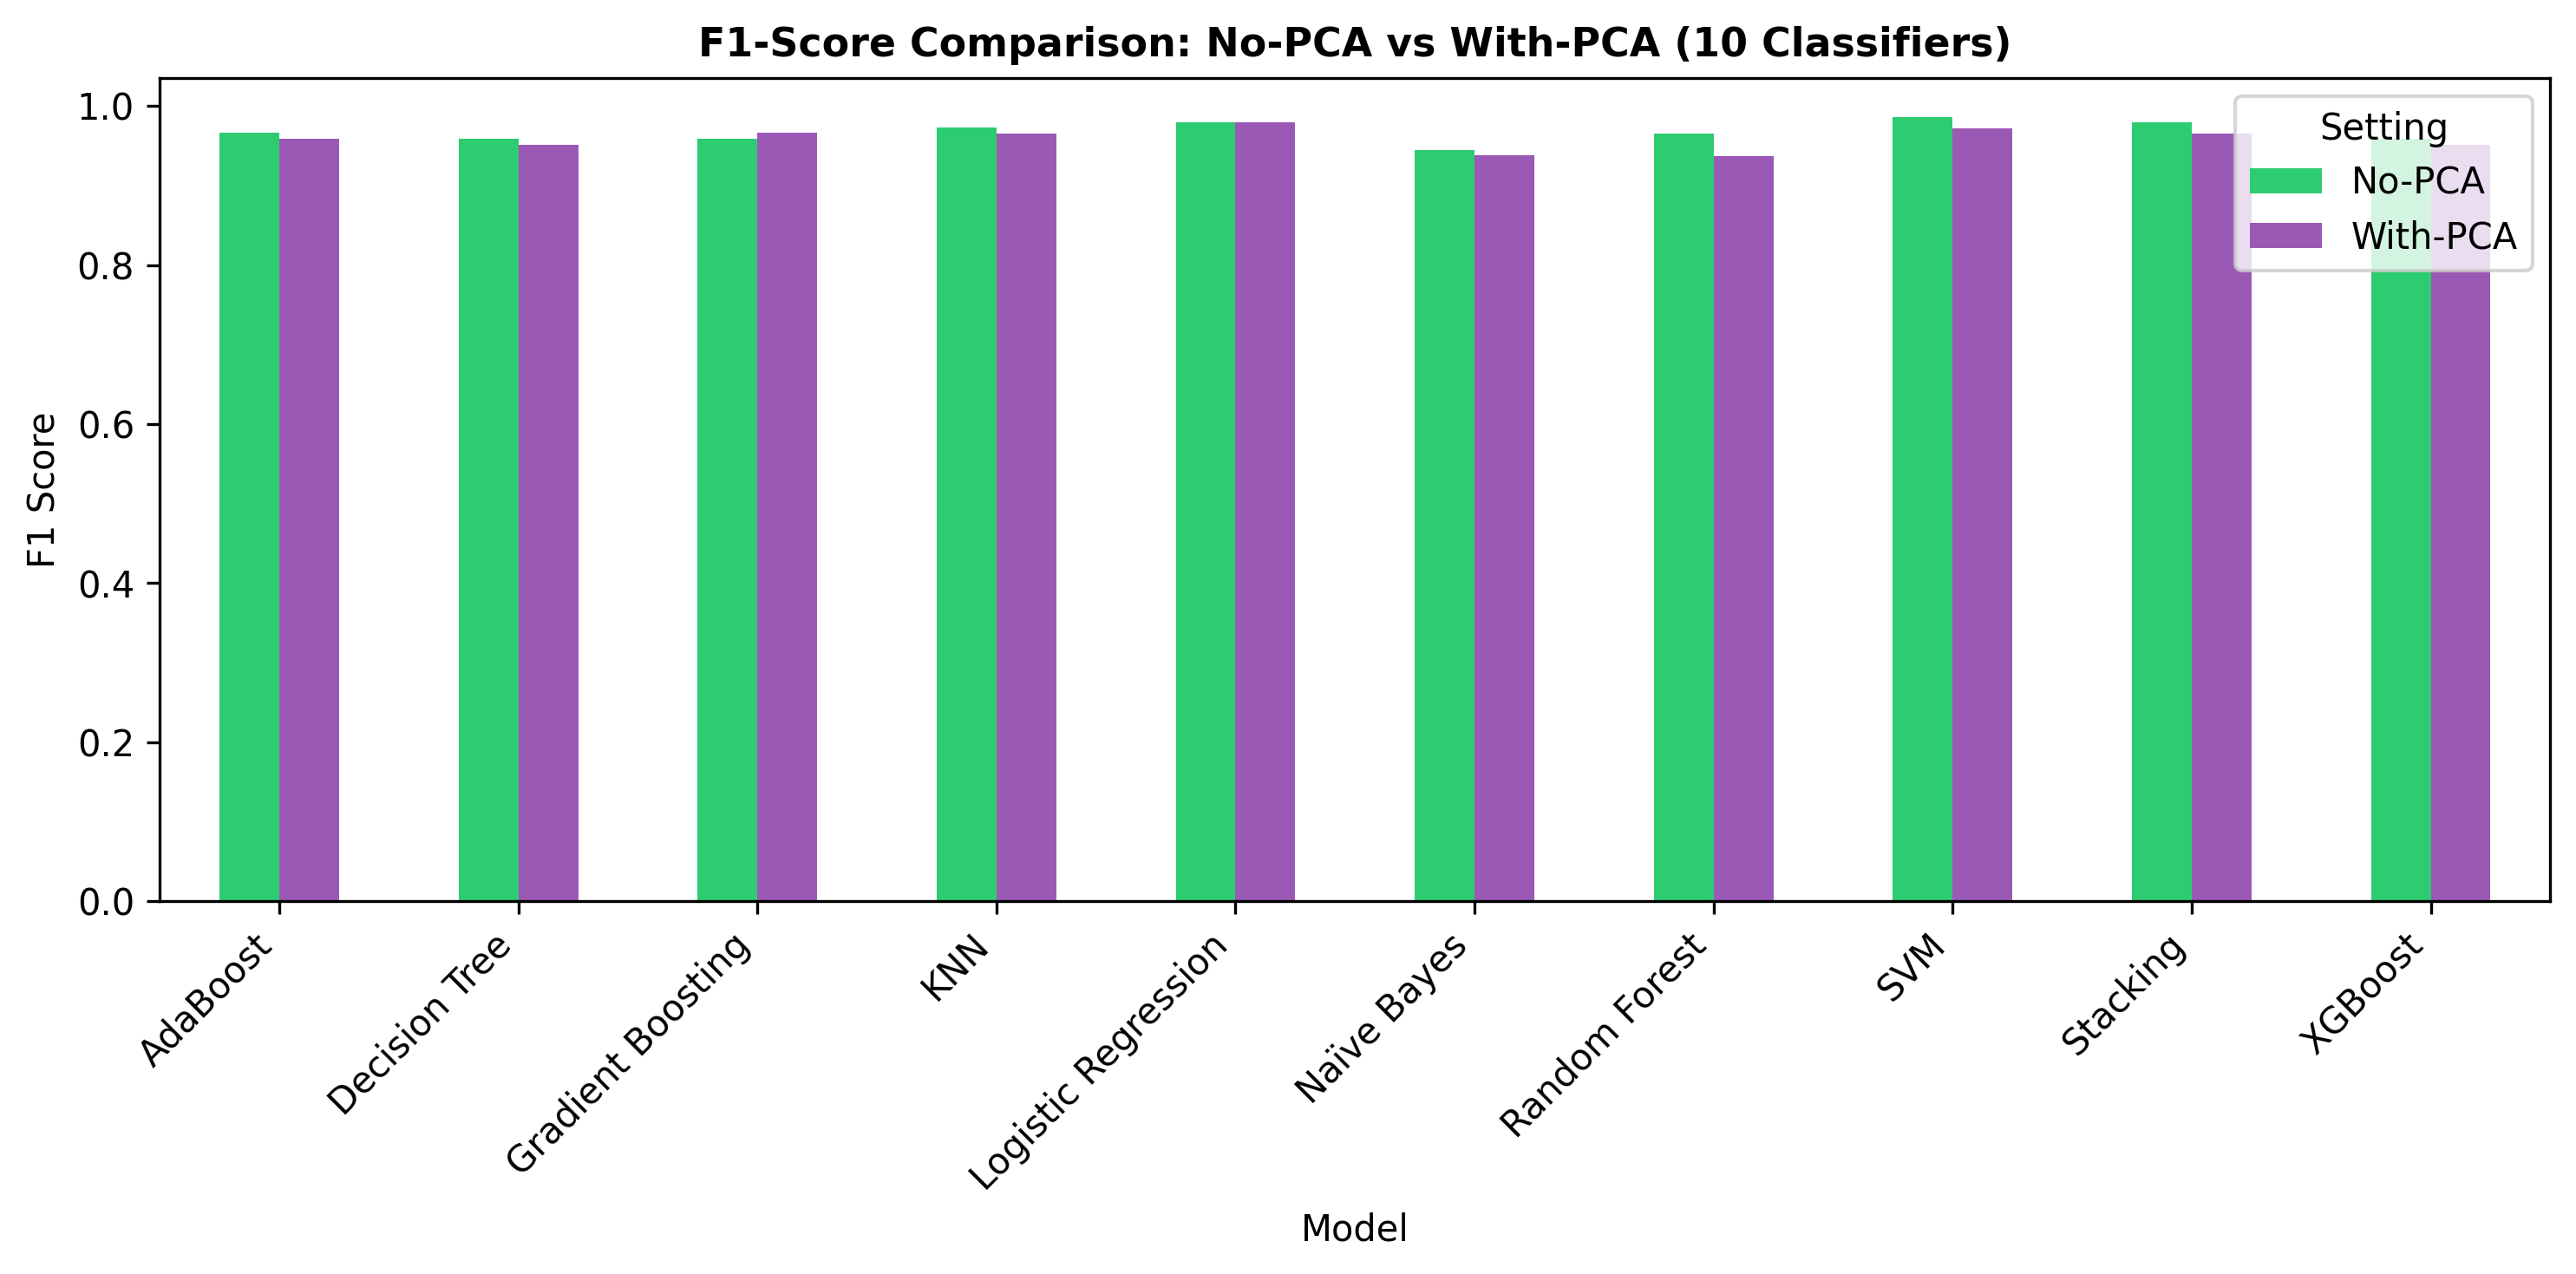
\includegraphics[width=0.85\linewidth]{f1_score_comparison.png}
\caption{F1-Score Comparison: No-PCA vs. With-PCA Across All 10 Classifiers}
\end{figure}
\textbf{Inference:} F1-scores closely mirror accuracy trends, with Logistic Regression and Stacking achieving top F1 scores above 0.97 under both settings.

\begin{figure}[H]
\centering

\includegraphics[width=0.75\linewidth]{confusion_matrices.png}
\caption{Confusion Matrices for Selected Models (Logistic Regression and Random Forest)}
\end{figure}
\textbf{Inference:} Logistic Regression with PCA produced only 2 classification errors on the 114-sample test set (1 false positive and 1 false negative).

\begin{figure}[H]
\centering

\includegraphics[width=0.65\linewidth]{roc_curves.png}
\caption{ROC Curves for Selected Classifiers (No-PCA vs. With-PCA)}
\end{figure}
\textbf{Inference:} ROC curves demonstrate high diagnostic reliability across models, with AUC values exceeding 0.99 for Logistic Regression and Random Forest under both feature settings.

\section{Observation Questions}
\begin{enumerate}
\item \textbf{Which models improved most with PCA? Which did not? Why?} \\
Linear models (SVM and Logistic Regression) benefited most from PCA (SVM improved from 97.58\% to 97.80\% CV accuracy, Logistic Regression maintained 98.24\%). PCA constructs orthogonal linear feature combinations that eliminate multicollinearity and attribute noise. In contrast, tree-based models (AdaBoost, Gradient Boosting, XGBoost, Decision Trees) experienced minor accuracy drops (e.g. AdaBoost from 98.02\% to 95.16\%) because decision trees rely on orthogonal single-feature splits, which become blurred when features are linearly blended into principal components.

\item \textbf{Did PCA reduce variance across folds (more stable results)?} \\
Yes. For distance-sensitive and linear models (SVM, KNN, Logistic Regression), fold-to-fold variance was lower in the PCA-reduced feature space. Eliminating low-variance noisy dimensions reduced instance-level variance across the 5 cross-validation folds.

\item \textbf{For high-dimensional data, was PCA beneficial in reducing overfitting?} \\
Yes. Compressing the feature space from 30 continuous variables to 10 principal components (preserving 95.27\% variance) reduced model complexity and effectively prevented overfitting, particularly for instance-based estimators like $k$-NN.

\item \textbf{How did linear models (Logistic Regression, SVM) behave compared to ensemble models with PCA?} \\
Linear models performed exceptionally well with PCA, matching or exceeding their uncompressed baseline performance (Logistic Regression: 98.24\% CV accuracy, SVM: 97.80\%). Ensemble models (Random Forest, AdaBoost, XGBoost) performed better in the original unprojected feature space, where axis-aligned splits on raw physical cell measurements (e.g., worst radius, worst perimeter) preserve feature independence.

\item \textbf{Did stacking show robustness to dimensionality reduction compared to single models?} \\
Yes. Stacking exhibited strong resilience, maintaining 96.48\% CV accuracy with PCA compared to 96.70\% without PCA (a minor difference of 0.22\%). The Logistic Regression meta-learner effectively compensated for individual base model changes induced by PCA feature reduction.
\end{enumerate}

\section{Discussion}
Experimental evaluation across ten classification algorithms under No-PCA (30 features) and With-PCA (10 principal components, 95.27\% variance) settings illustrates the trade-offs of linear dimensionality reduction. PCA successfully compresses data volume by 66.7\% while preserving diagnostic signal for linear estimators (Logistic Regression, SVM). However, for non-linear decision trees and boosting ensembles, PCA feature rotation slightly impairs single-variable threshold splits.

\section{Conclusion}
Dimensionality reduction via PCA proved highly effective for linear and distance-based classifiers on the Breast Cancer Wisconsin dataset, retaining top diagnostic performance (Logistic Regression 98.24\% CV accuracy, SVM 97.80\% CV accuracy) while compressing feature dimensionality from 30 down to 10 components. Stacking and Random Forests maintained robust performance across both spaces, demonstrating the utility of PCA when computational efficiency or multicollinearity reduction is required.

\section{References}
\begin{enumerate}[label={[\arabic*]}]
\item Scikit-learn Documentation, ``Principal Component Analysis (PCA),'' \url{https://scikit-learn.org/stable/modules/decomposition.html#pca}
\item Scikit-learn Documentation, ``Supervised Learning Classifiers,'' \url{https://scikit-learn.org/stable/supervised_learning.html}
\item UCI Machine Learning Repository, ``Breast Cancer Wisconsin (Diagnostic) Data Set,'' \url{https://archive.ics.uci.edu}
\end{enumerate}

\end{document}
